\documentclass{standalone}
\usepackage{tikz}
\usetikzlibrary{patterns, positioning}


\begin{document}
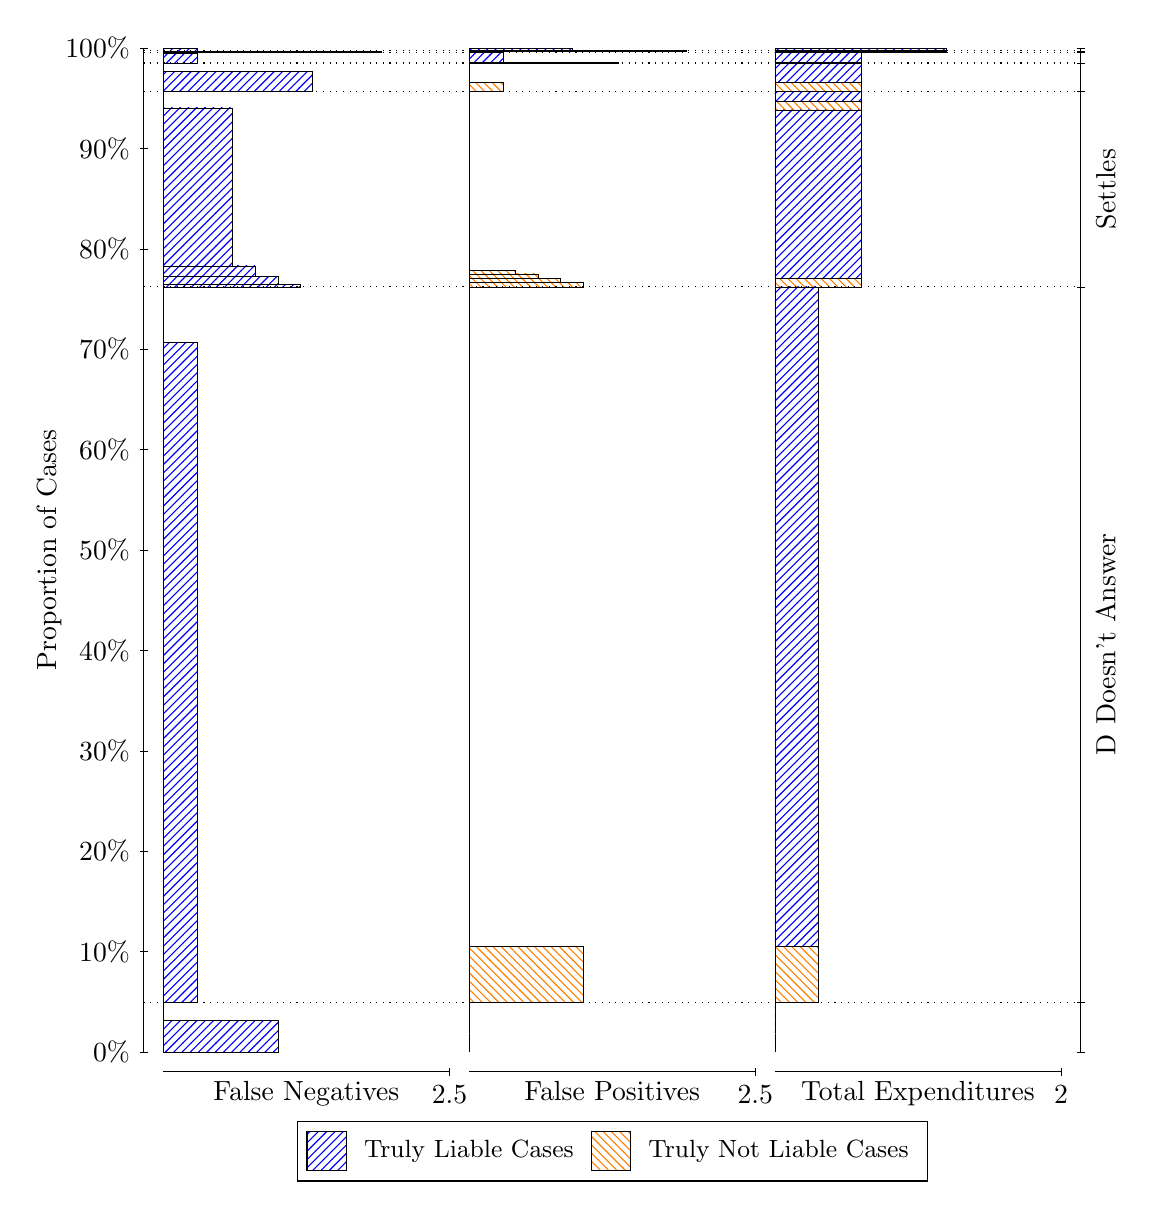
\begin{tikzpicture}
\draw[black, very thin] (1.5,1.75) -- (1.5,14.5);
\node[rotate=90, text=black, anchor=center] at (0.3, 8.125) {Proportion of Cases};
\draw[black, very thin] (1.45,1.75) -- (1.55,1.75);
\node[text=black, anchor=east] at (1.45, 1.75) {0\%};
\draw[black, very thin] (1.45,3.025) -- (1.55,3.025);
\node[text=black, anchor=east] at (1.45, 3.025) {10\%};
\draw[black, very thin] (1.45,4.3) -- (1.55,4.3);
\node[text=black, anchor=east] at (1.45, 4.3) {20\%};
\draw[black, very thin] (1.45,5.575) -- (1.55,5.575);
\node[text=black, anchor=east] at (1.45, 5.575) {30\%};
\draw[black, very thin] (1.45,6.85) -- (1.55,6.85);
\node[text=black, anchor=east] at (1.45, 6.85) {40\%};
\draw[black, very thin] (1.45,8.125) -- (1.55,8.125);
\node[text=black, anchor=east] at (1.45, 8.125) {50\%};
\draw[black, very thin] (1.45,9.4) -- (1.55,9.4);
\node[text=black, anchor=east] at (1.45, 9.4) {60\%};
\draw[black, very thin] (1.45,10.675) -- (1.55,10.675);
\node[text=black, anchor=east] at (1.45, 10.675) {70\%};
\draw[black, very thin] (1.45,11.95) -- (1.55,11.95);
\node[text=black, anchor=east] at (1.45, 11.95) {80\%};
\draw[black, very thin] (1.45,13.225) -- (1.55,13.225);
\node[text=black, anchor=east] at (1.45, 13.225) {90\%};
\draw[black, very thin] (1.45,14.5) -- (1.55,14.5);
\node[text=black, anchor=east] at (1.45, 14.5) {100\%};

\draw[black, very thin] (13.4,1.75) -- (13.4,14.5);
\draw[black, very thin] (13.35,1.75) -- (13.45,1.75);
\node[anchor=west] at (13.35, 1.75) {};
\draw[black, very thin] (13.35,2.3838) -- (13.45,2.3838);
\node[anchor=west] at (13.35, 2.3838) {};
\draw[black, very thin] (13.35,11.467) -- (13.45,11.467);
\node[anchor=west] at (13.35, 11.467) {};
\draw[black, very thin] (13.35,13.95) -- (13.45,13.95);
\node[anchor=west] at (13.35, 13.95) {};
\draw[black, very thin] (13.35,14.31) -- (13.45,14.31);
\node[anchor=west] at (13.35, 14.31) {};
\draw[black, very thin] (13.35,14.442) -- (13.45,14.442);
\node[anchor=west] at (13.35, 14.442) {};
\draw[black, very thin] (13.35,14.465) -- (13.45,14.465);
\node[anchor=west] at (13.35, 14.465) {};
\draw[black, very thin] (13.35,14.5) -- (13.45,14.5);
\node[anchor=west] at (13.35, 14.5) {};

\draw[black, very thin, pattern color=blue, pattern=north east lines] (1.75,1.75) rectangle (3.2033,2.1497);
\draw[black, very thin, pattern color=orange, pattern=north west lines] (1.75,2.1497) rectangle (1.75,2.3838);
\draw[black, very thin, pattern color=blue, pattern=north east lines] (1.75,2.3838) rectangle (2.186,10.764);
\draw[black, very thin, pattern color=orange, pattern=north west lines] (1.75,10.764) rectangle (1.75,11.467);
\draw[black, very thin, pattern color=blue, pattern=north east lines] (1.75,11.467) rectangle (3.494,11.495);
\draw[black, very thin, pattern color=blue, pattern=north east lines] (1.75,11.495) rectangle (3.3487,11.497);
\draw[black, very thin, pattern color=blue, pattern=north east lines] (1.75,11.497) rectangle (3.2033,11.597);
\draw[black, very thin, pattern color=blue, pattern=north east lines] (1.75,11.597) rectangle (2.9127,11.733);
\draw[black, very thin, pattern color=blue, pattern=north east lines] (1.75,11.733) rectangle (2.622,13.739);
\draw[black, very thin, pattern color=orange, pattern=north west lines] (1.75,13.739) rectangle (1.75,13.95);
\draw[black, very thin, pattern color=blue, pattern=north east lines] (1.75,13.95) rectangle (3.6393,14.201);
\draw[black, very thin, pattern color=orange, pattern=north west lines] (1.75,14.201) rectangle (1.75,14.31);
\draw[black, very thin, pattern color=blue, pattern=north east lines] (1.75,14.31) rectangle (2.186,14.431);
\draw[black, very thin, pattern color=orange, pattern=north west lines] (1.75,14.431) rectangle (1.75,14.442);
\draw[black, very thin, pattern color=blue, pattern=north east lines] (1.75,14.442) rectangle (4.5113,14.46);
\draw[black, very thin, pattern color=orange, pattern=north west lines] (1.75,14.46) rectangle (1.75,14.465);
\draw[black, very thin, pattern color=blue, pattern=north east lines] (1.75,14.465) rectangle (2.186,14.498);
\draw[black, very thin, pattern color=orange, pattern=north west lines] (1.75,14.498) rectangle (1.75,14.5);
\draw[black, very thin, pattern color=orange, pattern=north west lines] (5.6333,1.75) rectangle (5.6333,1.9841);
\draw[black, very thin, pattern color=blue, pattern=north east lines] (5.6333,1.9841) rectangle (5.6333,2.3838);
\draw[black, very thin, pattern color=orange, pattern=north west lines] (5.6333,2.3838) rectangle (7.0867,3.0868);
\draw[black, very thin, pattern color=blue, pattern=north east lines] (5.6333,3.0868) rectangle (5.6333,11.467);
\draw[black, very thin, pattern color=orange, pattern=north west lines] (5.6333,11.467) rectangle (7.0867,11.522);
\draw[black, very thin, pattern color=orange, pattern=north west lines] (5.6333,11.522) rectangle (6.796,11.573);
\draw[black, very thin, pattern color=orange, pattern=north west lines] (5.6333,11.573) rectangle (6.5053,11.632);
\draw[black, very thin, pattern color=orange, pattern=north west lines] (5.6333,11.632) rectangle (6.36,11.633);
\draw[black, very thin, pattern color=orange, pattern=north west lines] (5.6333,11.633) rectangle (6.2147,11.678);
\draw[black, very thin, pattern color=blue, pattern=north east lines] (5.6333,11.678) rectangle (5.6333,13.95);
\draw[black, very thin, pattern color=orange, pattern=north west lines] (5.6333,13.95) rectangle (6.0693,14.06);
\draw[black, very thin, pattern color=blue, pattern=north east lines] (5.6333,14.06) rectangle (5.6333,14.31);
\draw[black, very thin, pattern color=orange, pattern=north west lines] (5.6333,14.31) rectangle (7.5227,14.321);
\draw[black, very thin, pattern color=blue, pattern=north east lines] (5.6333,14.321) rectangle (6.0693,14.442);
\draw[black, very thin, pattern color=orange, pattern=north west lines] (5.6333,14.442) rectangle (6.0693,14.446);
\draw[black, very thin, pattern color=blue, pattern=north east lines] (5.6333,14.446) rectangle (5.6333,14.465);
\draw[black, very thin, pattern color=orange, pattern=north west lines] (5.6333,14.465) rectangle (8.3947,14.467);
\draw[black, very thin, pattern color=blue, pattern=north east lines] (5.6333,14.467) rectangle (6.9413,14.5);
\draw[black, very thin, pattern color=orange, pattern=north west lines] (9.5167,1.75) rectangle (9.5167,1.9841);
\draw[black, very thin, pattern color=blue, pattern=north east lines] (9.5167,1.9841) rectangle (9.5167,2.3838);
\draw[black, very thin, pattern color=orange, pattern=north west lines] (9.5167,2.3838) rectangle (10.062,3.0868);
\draw[black, very thin, pattern color=blue, pattern=north east lines] (9.5167,3.0868) rectangle (10.062,11.467);
\draw[black, very thin, pattern color=orange, pattern=north west lines] (9.5167,11.467) rectangle (10.607,11.573);
\draw[black, very thin, pattern color=blue, pattern=north east lines] (9.5167,11.573) rectangle (10.607,13.715);
\draw[black, very thin, pattern color=orange, pattern=north west lines] (9.5167,13.715) rectangle (10.607,13.82);
\draw[black, very thin, pattern color=blue, pattern=north east lines] (9.5167,13.82) rectangle (10.607,13.95);
\draw[black, very thin, pattern color=orange, pattern=north west lines] (9.5167,13.95) rectangle (10.607,14.06);
\draw[black, very thin, pattern color=blue, pattern=north east lines] (9.5167,14.06) rectangle (10.607,14.31);
\draw[black, very thin, pattern color=orange, pattern=north west lines] (9.5167,14.31) rectangle (10.607,14.321);
\draw[black, very thin, pattern color=blue, pattern=north east lines] (9.5167,14.321) rectangle (10.607,14.442);
\draw[black, very thin, pattern color=orange, pattern=north west lines] (9.5167,14.442) rectangle (11.697,14.446);
\draw[black, very thin, pattern color=blue, pattern=north east lines] (9.5167,14.446) rectangle (11.697,14.465);
\draw[black, very thin, pattern color=orange, pattern=north west lines] (9.5167,14.465) rectangle (11.697,14.467);
\draw[black, very thin, pattern color=blue, pattern=north east lines] (9.5167,14.467) rectangle (11.697,14.5);
\draw[black, dotted] (1.5,2.3838) -- (13.4,2.3838);
\draw[black, dotted] (1.5,11.467) -- (13.4,11.467);
\draw[black, dotted] (1.5,13.95) -- (13.4,13.95);
\draw[black, dotted] (1.5,14.31) -- (13.4,14.31);
\draw[black, dotted] (1.5,14.442) -- (13.4,14.442);
\draw[black, dotted] (1.5,14.465) -- (13.4,14.465);
\draw[black, very thin] (1.75,1.5) -- (5.3833,1.5);
\node[text=black, anchor=north] at (3.5667, 1.5) {False Negatives};
\draw[black, very thin] (5.3833,1.45) -- (5.3833,1.55);
\node[text=black, anchor=north] at (5.3833, 1.45) {2.5};

\draw[black, very thin] (5.6333,1.5) -- (9.2667,1.5);
\node[text=black, anchor=north] at (7.45, 1.5) {False Positives};
\draw[black, very thin] (9.2667,1.45) -- (9.2667,1.55);
\node[text=black, anchor=north] at (9.2667, 1.45) {2.5};

\draw[black, very thin] (9.5167,1.5) -- (13.15,1.5);
\node[text=black, anchor=north] at (11.333, 1.5) {Total Expenditures};
\draw[black, very thin] (13.15,1.45) -- (13.15,1.55);
\node[text=black, anchor=north] at (13.15, 1.45) {2};


\node[text=black, centered, rotate=90] at (13.72, 6.9255) {D Doesn't Answer};
\node[text=black, centered, rotate=90] at (13.72, 12.709) {Settles};





\draw (7.449999999999999,1.5) node[draw=none] (baseCoordinate) {};
\begin{scope}[align=center]
        \matrix[scale=0.5, draw=black, below=0.5cm of baseCoordinate, nodes={draw}, column sep=0.1cm]{
            \node[rectangle, draw, minimum width=0.5cm, minimum height=0.5cm, pattern color=blue, pattern=north east lines] {}; &
            \node[draw=none, font=\small, text=black] (B) {Truly Liable Cases}; &
            \node[rectangle, draw, minimum width=0.5cm, minimum height=0.5cm, pattern color=orange, pattern=north west lines] {}; &
            \node[draw=none, font=\small, text=black] (B) {Truly Not Liable Cases}; \\
            };
\end{scope}

\end{tikzpicture}
\end{document}